%第一段,在领域内的意义 
Due  to the increasing number of electronically-available publications stored in databases such as PubMed, there has been an increasing interest in applying text mining and information extraction to the medical literature. 
Medical literature mining has practical value for both medical research and applications. Medical named entity recognition and normalization are fundamental tasks in medical literature mining because the main developments in this area are usually related to these two.

%第二段,前人工作的缺陷
%Medical named entity recognition and normalization are to find the boundaries of mentions from the medical text and map them into a controlled vocabulary. State-of-the-art studies have demonstrated the superiority of joint modeling of medical named entity recognition and normalization compared to pipeline implementation due to mutual benefits between medical named entity recognition and normalization. There are two main disadvantages of those pipeline models: (1) errors from the recognition tagging cascade into normalization errors, and (2) recognition and normalization are both very useful for each other, but pipeline models cannot utilize these potential mutual benefits. Joint modeling recognition and normalization can naturally alleviate these two drawbacks and achieve state-of-the-art performance.   \citeauthor{Leaman2016TaggerOne} leveraged a joint scoring function for medical named entity recognition and normalization.  \citeauthor{Lou2017A} proposed a transition-based model to jointly perform medical named entity recognition and normalization, casting the output construction process into an incremental state transition process. However, these previous joint modeling methods 1) rely heavily on hand-crafted features and task specific resources; 2) use simple ways to jointly model medical named entity recognition and normalization.

The goal of medical named entity recognition and normalization is to find the boundaries of mentions from the medical text and map them onto a controlled vocabulary. State-of-the-art studies have demonstrated the superiority of joint modeling of medical named entity recognition and normalization compared to the pipeline implementation due to mutual benefits between them. There are two main disadvantages of pipeline models: (1) errors from the recognition tagging cascade into normalization errors, and (2) recognition and normalization are both very useful for each other, but pipeline models cannot utilize these potential benefits. Joint modeling recognition and normalization can naturally alleviate these two drawbacks and achieve state-of-the-art performance. \citeauthor{Leaman2016TaggerOne} (\citeyear{Leaman2016TaggerOne}) leveraged a joint scoring function for medical named entity recognition and normalization. \citeauthor{Lou2017A} (\citeyear{Lou2017A}) proposed a transition-based model to jointly perform medical named entity recognition and normalization, casting the output construction process into an incremental state transition process. However, these previous joint modeling methods (1) rely heavily on hand-crafted features and task specific resources thus fail to encode complicated and general features such as character-level and semantic-level features; 
(2) use simplistic ways to jointly model medical named entity recognition and normalization thus cannot model essential mutual supports between these two.   

%第三段,提出新方法及优点
%To improve the joint modeling medical named entity recognition and normalization, we propose a novel deep neural multi-task learning framework with explicit feedback strategies. This method can make use of the mutual benefits between recognition and normalization in a more advanced and intelligent way. On the one hand, our method benefits from general representations for both tasks via multi-task learning. The neural multi-task learning framework of our method benefits from a regularization effect that leads to more general representations to help both tasks, i.e., reducing over-fitting to a specific task, thus making the learned representations universal across tasks. 
%On the other hand, our method can successfully convert hierarchical tasks into parallel multi-task mode but maintains the mutual supports between tasks. Although the general concept of deep neural multi-task learning is not new, one novelty of our method is that it incorporates two feedback strategies from the low-level task to the high-level task and vice versa, as shown in Figure~\ref{fig: trans}. These two feedback strategies make it possible to convert hierarchical tasks into parallel multi-task mode but maintains the mutual supports between tasks. In addition, our method uses bi-directional RNNs to power the sequential modeling of the text and CNN to encode clues hided in character-level features such as \textbf{Zo}lmitriptan, \textbf{Zomig} and \textbf{Zomig}on.

To improve the joint modeling medical named entity recognition and normalization (MER and MEN), we propose a novel deep neural multi-task learning (MTL) framework with two explicit feedback strategies. This method can make use of the mutual benefits between recognition and normalization in a more advanced and intelligent way. First, our method benefits from general representations of both tasks provided by multi-task learning. The neural multi-task learning framework of our method benefits from a regularization effect~\cite{Collobert2011,DBLP:journals/corr/Ruder17a} that leads to more general representations to help both tasks. Specifically, it minimizes over-fitting to a specific task, thus making the learned representations universal across tasks. Second, our method can successfully convert hierarchical tasks into a parallel multi-task mode while maintaining mutual supports between tasks. Although the general concept of deep neural multi-task learning is not new, one innovation of our method is that it incorporates two feedback strategies from the low-level task to the high-level task and vice versa, as shown in Figure~\ref{fig: trans}. 
These two feedback strategies exploit the output of entity recognition to improve entity normalization and vice versa.
In addition, our method uses Bi-LSTM to power the sequential modeling of text and CNN to encode clues hidden in character-level features such as \textbf{Zo}lmitriptan, \textbf{Zomig} and \textbf{Zomig}on.
\begin{figure}[tp]
	\centering
	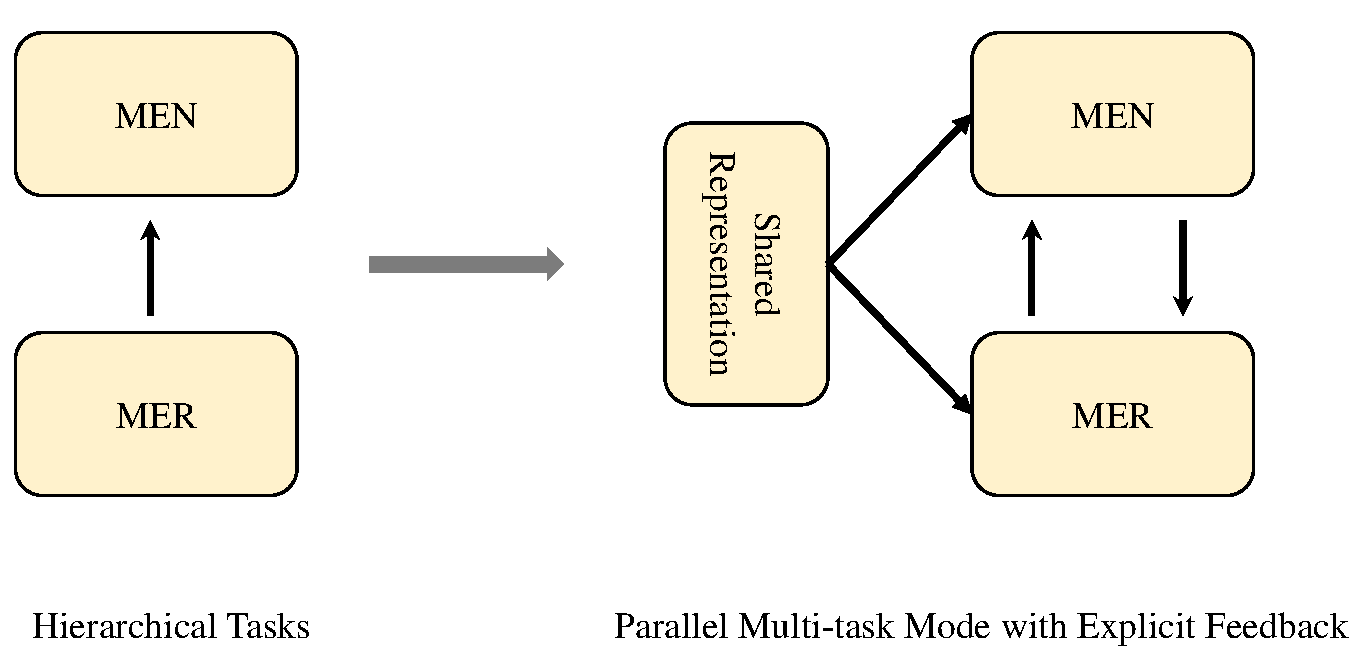
\includegraphics[width=0.4\textwidth]{fig/tranformation}
	\vspace{-0.1in}
	\caption{From hierarchical tasks to parallel multi-task mode by incorporating explicit feedback strategies among tasks. %MER refers to medical named entity recognition, MEN refers to medical named entity normalization.
		}\label{fig: trans}
	\vspace{-0.15in}
\end{figure}

We evaluate our models across two corpora (the BioCreative V Chemical Disease Relation (BC5CDR) task corpus \cite{Li2016BioCreative} and the NCBI Disease corpus \cite{Rezarta2014NCBI}) of medical articles and outperform the state-of-the-art study by up to 4.53\% F1 on medical named entity recognition and 5.61\% F1 on medical named entity normalization.



\textbf{Contribution.}
%In order to make use of the mutual benefits in a more advanced and intelligent way, we propose a novel deep neural multi-task learning framework with explicit feedback strategies to jointly model recognition and normalization. This method incorporates two feedback strategies from the low-level task to the high-level task and vice versa, making it possible to convert hierarchical tasks into parallel multi-task mode but maintains the mutual supports between tasks.
To make use of the mutual benefits in a more sophisticated way, we propose a novel deep neural multi-task learning framework with explicit feedback strategies to jointly model recognition and normalization. This method incorporates two feedback strategies from the low-level task to the high-level task and vice versa, making it possible to convert hierarchical tasks, i.e. MER and MEN, into parallel multi-task mode while maintaining mutual supports between tasks.
